% Here we include more details on all aspects in Section 2 if they can be useful for the development team.

\subsection{External Interface Requirements}

\subsubsection{User Interfaces}

% We need a tool, either stores raw content as text in our repo, or integrates with GitHub.
% TODO: @Ozan finish ui mockups

% Actual mockups of user interfaces

\subsubsection{Hardware Interfaces}
% TODO: @Hrvoje These 3
% Do we integrate with external hardware?
\subsubsection{Software Interfaces}

% Do we integrate with custom software, expose an API?

\subsubsection{Communication Interfaces}


% What is a communication interface? the Internet? RF port? Radio? Bluetooth?

\subsection{Functional Requirements}
% Use draw.io, compatible with GitHub.
% TODO: @Ozan Embed stuff here

% TODO: @Roberto finish the table and sequence diagrams
% Definition  of  use  case  diagrams,  use  cases  and  associated sequence/activity diagrams, and mapping on requirements

% Use case diagram

% For each use case:
%   Use case table
%   Use case sequence diagram
\subsubsection{Customer}

\begin{figure}[H]
    \centering
    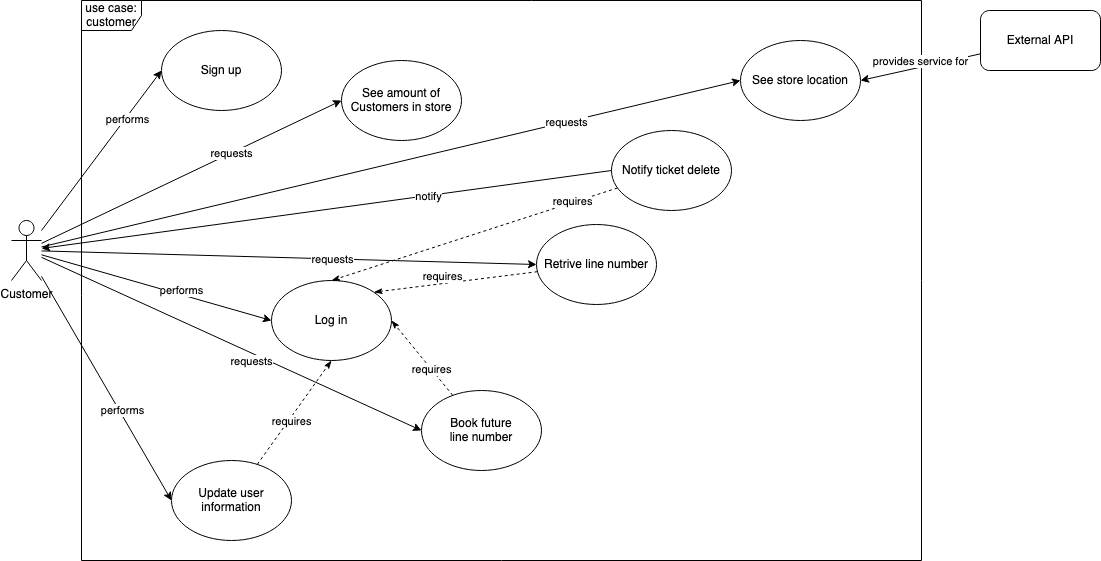
\includegraphics[width=\textwidth]{Images/UseCaseDiagrams/Customer.png}
    \caption{Use Case Diagram for Customer}
\end{figure}
\textbf{Use cases}
\begin{table}[H]
    \begin{tabular}{|p{8cm}|p{8cm}|}
        \hline
        \textit{Name}    & \textbf{Book future line number} \\ \hline
        \textit{Actors} & Customer \\ \hline
        \textit{Entry conditions} & The customer is logged in the app and wants to book a visit to the store. \\ \hline
        \textit{Event flows}      & \tabitem The customer clicks on the "Book a Visit" button in the app. \\
        & \tabitem The app asks the time slot and the estimated time of the visit presenting as default value the average of the previous times of visit of the same user. \\
        & \tabitem The customer sets the time slot and the estimated time of their visit. \\
        & \tabitem The app asks what category of products the customer wants to buy. \\
        & \tabitem The customer set the products categories. \\
        & \tabitem The app requests the line number from the server. \\
        & \tabitem The app generates the QR code on the response from the server. \\
        \hline
        \textit{Exit conditions} & The customer has booked a visit for the store. \\ \hline
        \textit{Exceptions} & \tabitem The server cannot retrieve the line number since the time slot is full.\\ \hline
    \end{tabular}
    \caption{Use Case: Book future line number}
\end{table}
\begin{figure}[H]
    \centering
    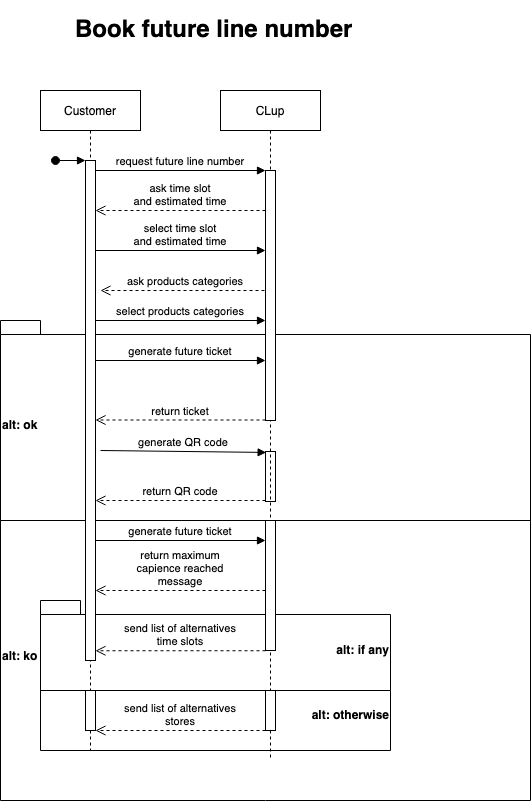
\includegraphics[width=\textwidth]{Images/SequenceDiagrams/Customer/BookFutureLineNumberUseCaseSequenceDiagram.png}
    \caption{Sequence Diagram for Use Case: Book future line number}
\end{figure}
\begin{table}[H]
    \begin{tabular}{|p{8cm}|p{8cm}|}
        \hline
        \textit{Name}    & \textbf{See amount of customers in the store} \\ \hline
        \textit{Actors} & Customer \\ \hline
        \textit{Entry conditions} & The customer is logged in the app and wants to know how many customers are in the store in order to decide whether to book a visit or retrieve a line number \\ \hline
        \textit{Event flows}      & \tabitem The customer clicks on the  "Live Store Info" button. \\
        & \tabitem The app sends a count request to the server. \\
        & \tabitem The server returns the live data for the amount of customers in the store for each time slot. \\
        \hline
        \textit{Exit conditions} & The customer knows the amount of customers in the store and can plan their visit. \\ \hline
        \textit{Exceptions} & \\ \hline
    \end{tabular}
    \caption{Use Case: See amount of customers in the store}
\end{table}
\begin{figure}[H]
    \centering
    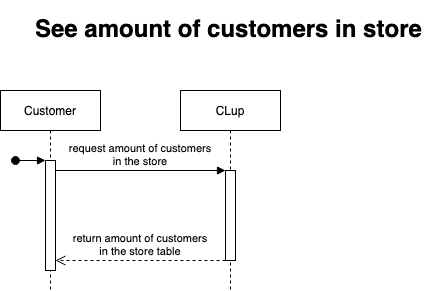
\includegraphics[width=\textwidth]{Images/SequenceDiagrams/Customer/SeeAmountOfCustomersInStoreUseCaseSequenceDiagram.png}
    \caption{Sequence Diagram for Use Case: See amount of customers in the store}
\end{figure}
\begin{table}[H]
    \begin{tabular}{|p{8cm}|p{8cm}|}
        \hline
        \textit{Name}    & \textbf{See store location} \\ \hline
        \textit{Actors} & Customer, Maps API \\ \hline
        \textit{Entry conditions} & The customer needs to know where the store is located and the travel time \\ \hline
        % TODO: Are entry conditions things already met (user logged in) or intention (Customer wants, needs etc...)
        \textit{Event flows}      & \tabitem The customer clicks on the "Store Location" button. \\
        & \tabitem The app contacts the Maps API with the store location. \\
        & \tabitem The Maps API returns a map from the customer position to the store with a time estimation. \\
        \hline
        \textit{Exit conditions} & The customer knows how to go to the store and the travel time needed. \\ \hline
        \textit{Exceptions} & \tabitem The customer's smartphone doesn't provide or allow access to location services. \\
        \hline
    \end{tabular}
    \caption{Use Case: See store location}
\end{table}
\begin{figure}[H]
    \centering
    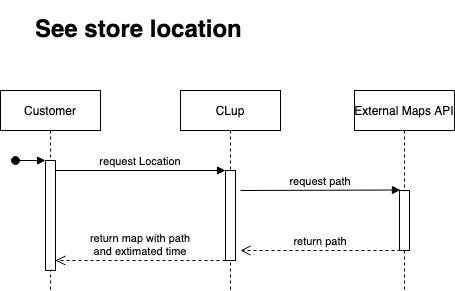
\includegraphics[width=\textwidth]{Images/SequenceDiagrams/Customer/SeeStoreLocationUseCaseSequenceDiagram.png}
    \caption{Sequence Diagram for Use Case: See store location}
\end{figure}

\begin{table}[H]
    \begin{tabular}{|p{8cm}|p{8cm}|}
        \hline
        \textit{Name}    & \textbf{Sign up} \\ \hline
        \textit{Actors} & Customer \\ \hline
        \textit{Entry conditions} & The customer opened the app and they are not registered yet, and they want to register. \\ \hline
        \textit{Event flows}      & \tabitem The customer clicks on the "Sign Up" button. \\
        & \tabitem The customer inserts their credentials. \\
        & \tabitem The app sends the information to the server. \\
        & \tabitem The server stores the data related to the user. \\
        & \tabitem The server returns an acknowledgement to the app. \\
        \hline
        \textit{Exit conditions} & The customer is now registered and can use all the functionalities of the app. \\ \hline
        \textit{Exceptions} & \tabitem The e-mail provided in the registration form is already used by another user. \\
        & \tabitem The credentials provided in the registration form are ill-formatted.\\
        \hline
    \end{tabular}
    \caption{Use Case: Sign up}
\end{table}

\begin{figure}[H]
    \centering
    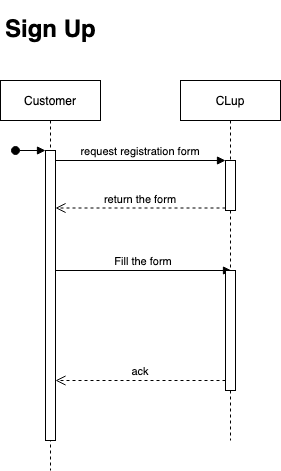
\includegraphics[width=\textwidth]{Images/SequenceDiagrams/Customer/SignUpUseCaseSequenceDiagram.png}
    \caption{Sequence Diagram for Use Case: Sign up}
\end{figure}

\begin{table}[H]
    \begin{tabular}{|p{8cm}|p{8cm}|}
        \hline
        \textit{Name}    & \textbf{Login} \\ \hline
        \textit{Actors} & User \\ \hline
        \textit{Entry conditions} & The user has already sign up and wants to login to use CLup functionalities \\ \hline
        \textit{Event flows}     & \tabitem The customer clicks on the "Login" button\\
        & \tabitem The user provides their login credentials. \\
        & \tabitem The system authenticates the user \\
        \hline
        \textit{Exit conditions} & The user is logged in and can now use all the CLup functionalities \\ \hline
        \textit{Exceptions} & \tabitem The credentials are wrong \\
        \hline
    \end{tabular}
    \caption{Use Case: Login}
\end{table}

\begin{figure}[H]
    \centering
    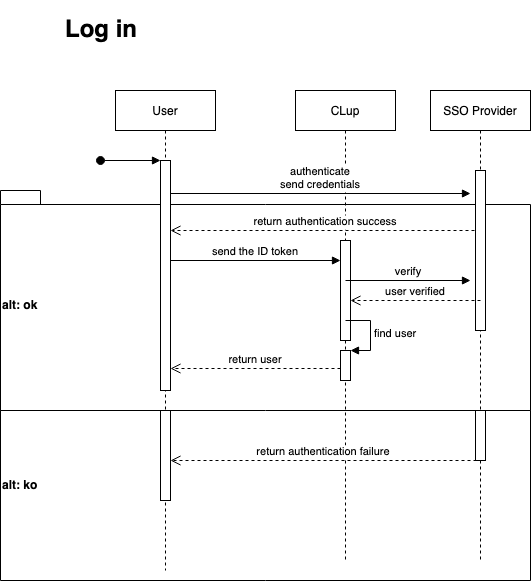
\includegraphics[width=\textwidth]{Images/SequenceDiagrams/LogInUseCaseSequenceDiagram.png}
    \caption{Sequence Diagram for Use Case: Login}
\end{figure}

\begin{table}[H]
    \begin{tabular}{|p{8cm}|p{8cm}|}
        \hline
        \textit{Name}    & \textbf{Notify ticket delete} \\ \hline
        \textit{Actors} & Customer \\ \hline
        \textit{Entry conditions} & A ticket of the Customer was deleted from the server. \\ \hline
        \textit{Event flows}     & \tabitem The system sends an email to the customer to notify the deletion of their ticket\\
        \hline
        \textit{Exit conditions} & The customer is informed about the deletion of their ticket. \\ \hline
        \textit{Exceptions} & \tabitem \\
        \hline
    \end{tabular}
    \caption{Use Case: Notify ticket delete}
\end{table}

\begin{figure}[H]
    \centering
    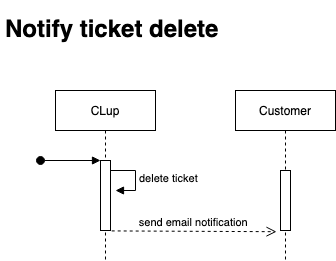
\includegraphics[width=\textwidth]{Images/SequenceDiagrams/Customer/NotifyTicketDeleteUseCaseSequenceDiagram.png}
    \caption{Sequence Diagram for Use Case: Notify ticket delete}
\end{figure}

\begin{table}[H]
    \begin{tabular}{|p{8cm}|p{8cm}|}
        \hline
        \textit{Name}    & \textbf{Update user information} \\ \hline
        \textit{Actors} & User \\ \hline
        \textit{Entry conditions} & The user wants to change an information of themselves. \\ \hline
        \textit{Event flows}     & \tabitem The user clicks on the "Update User Information" button. \\
        & \tabitem The app shows a form precompiled with user's previous information. \\
        & \tabitem The user changes the information on the respective fields and presses the "Submit" button. \\
        & \tabitem The system saves the changes. \\
        \hline
        \textit{Exit conditions} & The user successfully updated their information. \\ \hline
        \textit{Exceptions} & \tabitem The new information provided is ill-formatted. \\
        \hline
    \end{tabular}
    \caption{Use Case: Update user information}
\end{table}

\begin{figure}[H]
    \centering
    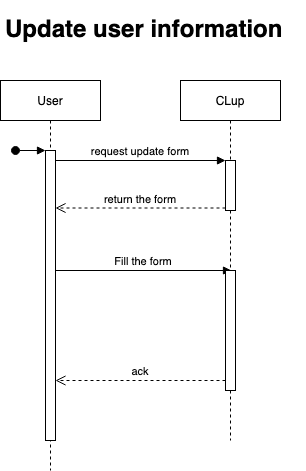
\includegraphics[width=\textwidth]{Images/SequenceDiagrams/UpdateUserInformationUseCaseSequenceDiagram.png}
    \caption{Sequence Diagram for Use Case: Update user information}
\end{figure}

\subsubsection{Clerk}

\begin{figure}[H]
    \centering
    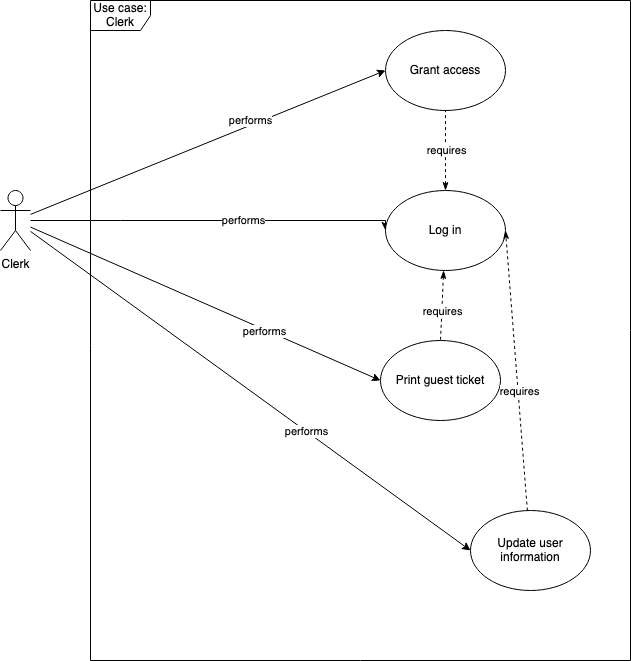
\includegraphics[width=\textwidth]{Images/UseCaseDiagrams/Clerk.png}
    \caption{Use Case Diagram for Clerk}
\end{figure}

\textbf{Use cases}

\begin{table}[H]
    \begin{tabular}{|p{8cm}|p{8cm}|}
        \hline
        \textit{Name}    & \textbf{Grant access} \\ \hline
        \textit{Actors} & Clerk, Customer \\ \hline
        \textit{Entry conditions} & The customer has already obtained the QR code and they plan on entering the store.\\ \hline
        \textit{Event flows}      & \tabitem The Clerk scans the QR code from the customer's smartphone or printed ticket using the app \\
        & \tabitem The app analyzes the QR code and contacts to the Server \\
        & \tabitem The server decides if the customer can enter based on the information received in the QR code \\
        & \tabitem The server responds to the clerk app with the result \\
        & \tabitem The clerk let the customer enter the store \\ % TODO: Are we supposed to write about world phenomena?
        \\ \hline
        \textit{Exit conditions} & The customer enters the store \\ \hline
        \textit{Exceptions} & \tabitem The server communicates to the clerk that the customer cannot enter because their line number is not available.\\ \hline
    \end{tabular}
    \caption{Use Case: Grant access}
\end{table}

\begin{figure}[H]
    \centering
    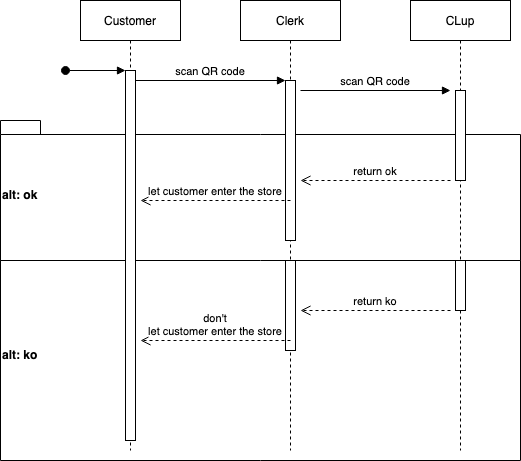
\includegraphics[width=\textwidth]{Images/SequenceDiagrams/Clerk/GrantAccessUseCaseSequenceDiagram.png}
    \caption{Sequence Diagram for Use Case: Update user information}
\end{figure}

\begin{table}[H]
    \begin{tabular}{|p{8cm}|p{8cm}|}
        \hline
        \textit{Name}    & \textbf{Print guest ticket} \\ \hline
        \textit{Actors} & Clerk, Customer \\ \hline
        \textit{Entry conditions} & The customer has arrived to the location, doesn't have a ticket on their smartphone, and needs a physical ticket to enter. \\ \hline
        \textit{Event flows}      & \tabitem The customer asks the clerk for a ticket. \\
        & \tabitem The clerk generate a ticket using the app. \\
        & \tabitem The app sends a request to the server to generate a ticket. \\
        & \tabitem The server generates a line number and a ticket. \\
        & \tabitem The server sends the ticket back to the app. \\
        & \tabitem The clerk prints the ticket. \\ % TODO: Real world phenomena here again?
        & \tabitem The clerk gives the ticket to the customer. \\
        \hline
        \textit{Exit conditions} & The customer has a ticket. \\ \hline
        \textit{Exceptions} & \tabitem The server cannot generate a line number due to capacity constraints. \\ \hline
    \end{tabular}
    \caption{Use Case: Print guest ticket}
\end{table}

\begin{figure}[H]
    \centering
    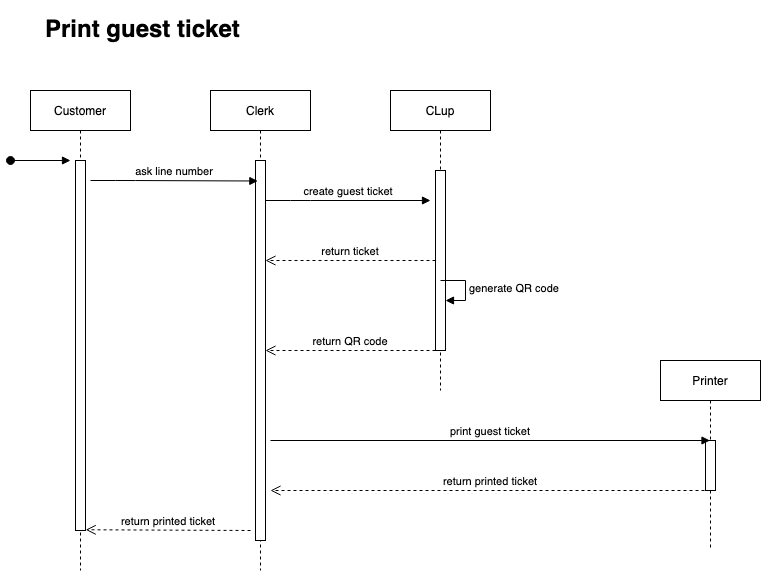
\includegraphics[width=\textwidth]{Images/SequenceDiagrams/Clerk/PrintGuestTicketUseCaseSequenceDiagram.png}
    \caption{Sequence Diagram for Use Case: Print guest ticket}
\end{figure}

\subsubsection{Manager}

\begin{figure}[H]
    \centering
    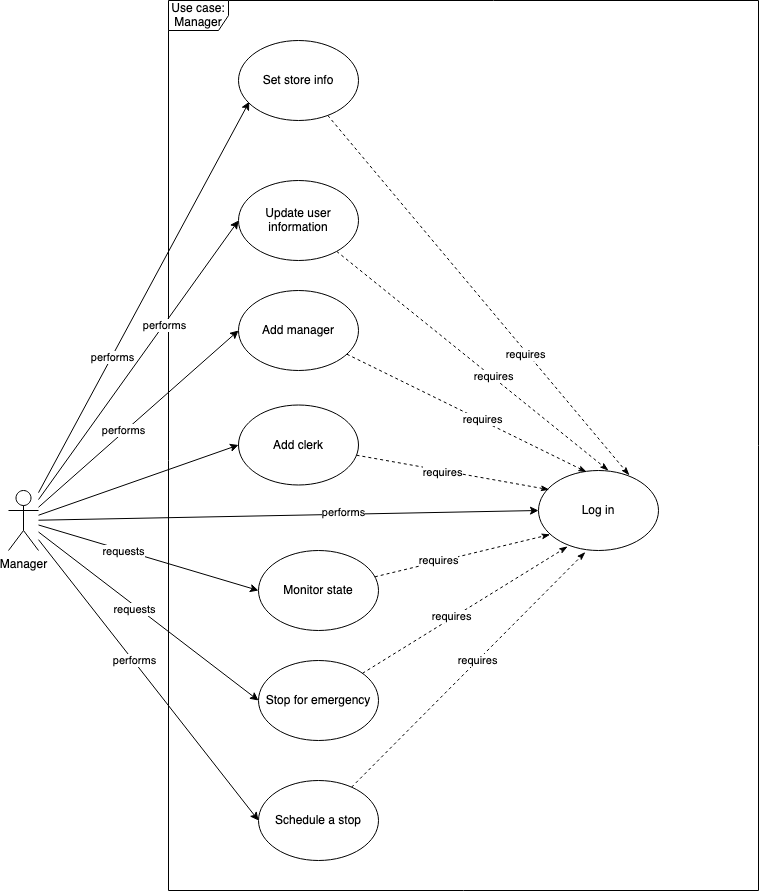
\includegraphics[width=\textwidth]{Images/UseCaseDiagrams/Manager.png}
    \caption{Use Case Diagram for Manager}
\end{figure}

\textbf{Use cases}

\begin{table}[H]
    \begin{tabular}{|p{8cm}|p{8cm}|}
        \hline
        \textit{Name}    & \textbf{Initialize} \\ \hline
        \textit{Actors} & Manager \\ \hline
        \textit{Entry conditions} & The manager of the store needs to set the basic information of the store in order to start the service \\ \hline
        \textit{Event flows}      & \tabitem The manager clicks on the initialize button \\
        & \tabitem The app shows the location form to the manager \\
        & \tabitem The manager fills the form and sends ıt to the server via the app\\
        & \tabitem The server registers the information and acknowledges \\
        \hline
        \textit{Exit conditions} & The system is initialized and can offer all its functions \\ \hline
        \textit{Exceptions} & \tabitem Some mandatory parts of the form are not filled. \\ \hline
    \end{tabular}
    \caption{Use Case: Initialize}
\end{table}

% TODO: There is no request for info form, front-end is capable of generating such info.
\begin{figure}[H]
    \centering
    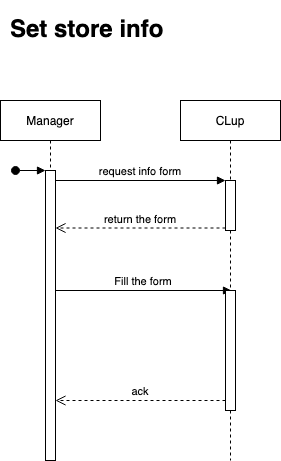
\includegraphics[width=\textwidth]{Images/SequenceDiagrams/Manager/SetStoreInfoUseCaseSequenceDiagram.png}
    \caption{Sequence Diagram for Use Case: Initialize}
\end{figure}

\begin{table}[H]
    \begin{tabular}{|p{8cm}|p{8cm}|}
        \hline
        \textit{Name}    & \textbf{Monitor state} \\ \hline
        \textit{Actors} & Manager \\ \hline
        \textit{Entry conditions} & The manager wants to monitor the number of customers in the store in real time. \\ \hline
        \textit{Event flows}      & \tabitem The manager clicks on the "Monitoring" button. \\
        & \tabitem The app sends the number request to the server.  \\
        & \tabitem The server returns the number of customers in the store. \\
        & \tabitem The app repeats the process periodically as long as the monitoring page is open. \\ % TODO: What period? Do we need to specify this?
        \hline
        \textit{Exit conditions} & The manager is informed on the number of the customers in the store in real time. \\ \hline
        \textit{Exceptions} & \tabitem \\ \hline
    \end{tabular}
    \caption{Use Case: Monitor state}
\end{table}

\begin{figure}[H]
    \centering
    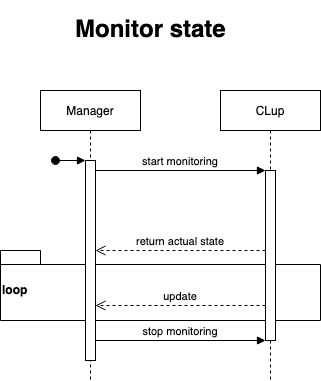
\includegraphics[width=\textwidth]{Images/SequenceDiagrams/Manager/MonitorStateUseCaseSequenceDiagram.png}
    \caption{Sequence Diagram for Use Case: Monitor state}
\end{figure}

\begin{table}[H]
    \begin{tabular}{|p{8cm}|p{8cm}|}
        \hline
        \textit{Name}    & \textbf{Schedule a stop} \\ \hline
        \textit{Actors} & Manager \\ \hline
        \textit{Entry conditions} & The manager wants to schedule a period of time in which the store will be closed so the users can not book a visit for that time. \\ \hline
        \textit{Event flows}      & \tabitem The manager clicks on the "Schedule a Stop" button. \\
        & \tabitem The app shows a form for the time of the stop. \\
        & \tabitem The manager fills the form and submits it to the server through the app. \\
        & \tabitem The server stores the information in the database and returns an acknowledgement. \\
        \hline
        \textit{Exit conditions} & The system has a scheduled stop stored in its database and will use it to prevent customers from booking a visit in that time period. \\ \hline
        \textit{Exceptions} & \tabitem There is already a planned stop in that period. \\ \hline
    \end{tabular}
    \caption{Use Case: Schedule a stop}
\end{table}

\begin{figure}[H]
    \centering
    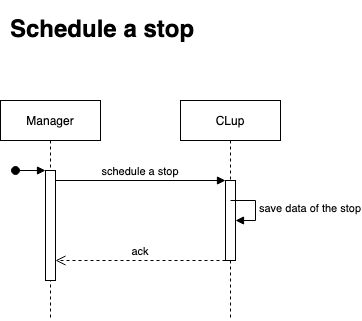
\includegraphics[width=\textwidth]{Images/SequenceDiagrams/Manager/ScheduleAStopUseCaseSequenceDiagram.png}
    \caption{Sequence Diagram for Use Case: Schedule a stop}
\end{figure}

\begin{table}[H]
    \begin{tabular}{|p{8cm}|p{8cm}|}
        \hline
        \textit{Name}    & \textbf{Stop for emergency} \\ \hline
        \textit{Actors} & Manager \\ \hline
        \textit{Entry conditions} & An emergency occurred and the manager wants to immediately stop the system from distributing line numbers. \\ \hline
        \textit{Event flows}     & \tabitem The manager click on the "Emergency Stop" button \\
        & \tabitem The app asks for confirmation from the manager. \\
        & \tabitem The manager confirms the stop of the system. \\
        & \tabitem The app sends the system stop request to the server. \\
        & \tabitem The server stops the service and return an acknowledgement. \\
        \hline
        \textit{Exit conditions} & The system has interrupted the service. \\ \hline
        \textit{Exceptions} & \tabitem The manager aborts the operation. \\
        \hline
    \end{tabular}
    \caption{Use Case: Stop for emergency}
\end{table}

\begin{figure}[H]
    \centering
    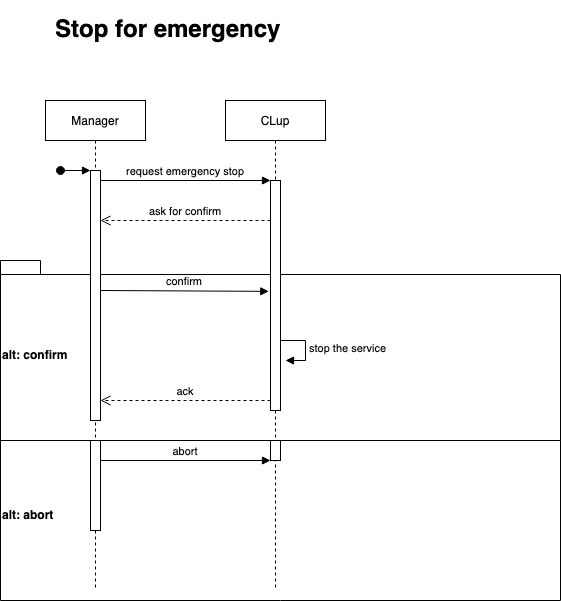
\includegraphics[width=\textwidth]{Images/SequenceDiagrams/Manager/StopForEmergencyUseCaseSequenceDiagram.png}
    \caption{Sequence Diagram for Use Case: Stop for emergency}
\end{figure}

\begin{table}[H]
    \begin{tabular}{|p{8cm}|p{8cm}|}
        \hline
        \textit{Name}    & \textbf{Add Clerk} \\ \hline
        \textit{Actors} & Manager \\ \hline
        \textit{Entry conditions} & The manager wants to add a new clerk to the system \\ \hline
        \textit{Event flows}     & \tabitem The manager click on the "add clerk" button \\
        & \tabitem The system asks the data of the new clerk (e.g. the credentials) \\
        & \tabitem The manager inserts the data and press "submit" \\
        \hline
        \textit{Exit conditions} & The new clerk is added to the system \\ \hline
        \textit{Exceptions} & \tabitem The data of the clerk are incomplete or incorrect \\
        \hline
    \end{tabular}
    \caption{Use Case: Add Clerk}
\end{table}

\begin{figure}[H]
    \centering
    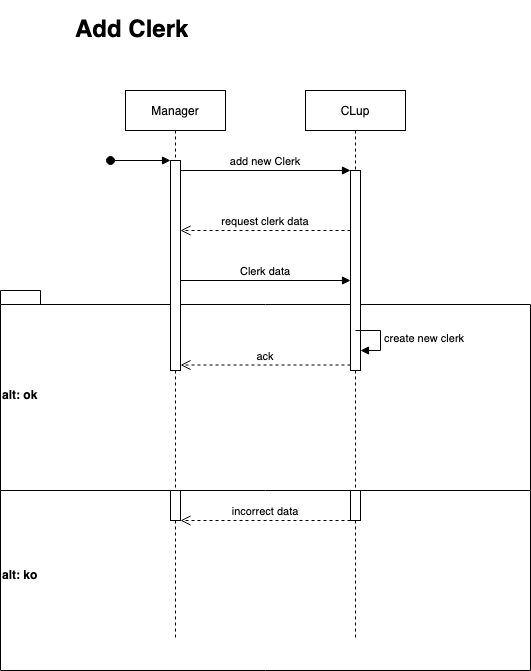
\includegraphics[width=\textwidth]{Images/SequenceDiagrams/Manager/AddClerkUseCaseSequenceDiagram.png}
    \caption{Sequence Diagram for Use Case: Add Clerk}
\end{figure}

\begin{table}[H]
    \begin{tabular}{|p{8cm}|p{8cm}|}
        \hline
        \textit{Name}    & \textbf{Add Manager} \\ \hline
        \textit{Actors} & Manager \\ \hline
        \textit{Entry conditions} & The manager wants to add a new manager to the system \\ \hline
        \textit{Event flows}     & \tabitem The manager click on the "Add Manager" button \\
        & \tabitem The system asks the data of the new manager (e.g. the credentials) \\
        & \tabitem The manager inserts the data and press "Submit" \\
        \hline
        \textit{Exit conditions} & The new Manager is added to the system \\ \hline
        \textit{Exceptions} & \tabitem The data of the Manager are incomplete or incorrect \\
        \hline
    \end{tabular}
    \caption{Use Case: Add Manager}
\end{table}

\begin{figure}[H]
    \centering
    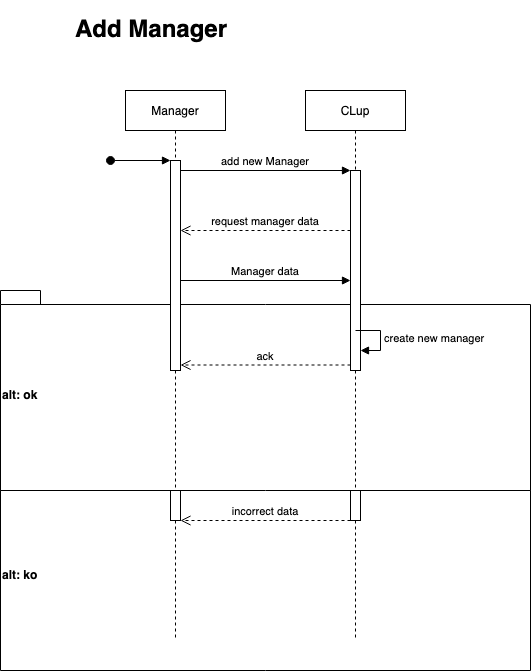
\includegraphics[width=\textwidth]{Images/SequenceDiagrams/Manager/AddManagerUseCaseSequenceDiagram.png}
    \caption{Sequence Diagram for Use Case: Add Manager}
\end{figure}

\subsubsection{Requirements}
\begin{itemize}
    \item \textbf{$R_1$} The system must allow users to authenticate using their e-mail address and password. % TODO: Roberto add use case
    \item \textbf{$R_2$} The system must allow customers to register using their e-mail address, their name, surname, phone number and a new password.
    \item \textbf{$R_3$} The system must provide a hard-coded super user to allow addition of locations and managers of locations.
    \item \textbf{$R_4$} Managers must be able to add additional managers and clerks as users.
    \item \textbf{$R_5$} Managers must be able to set and update location specific information, that are maximum number of customers in the location at any given time, opening and closing hours of the store per each day, line number timeout, limit of reservation per customer on a predetermined time interval that is one of month, week or day, and location of the place % One form
    \item \textbf{$R_6$} Managers can add any other location as a partner store.
    \item \textbf{$R_7$} Managers can stop the system from issuing any more tickets for a given day
    \item \textbf{$R_8$} Managers can schedule the system stop for a future time.
    \item \textbf{$R_9$} Managers can set the in-shop locations for different categories and product items.
    \item \textbf{$R_{10}$} In case of a system stop, no further line numbers can be issued for the given time slots.
    \item \textbf{$R_{11}$} In case of a system stop, all line numbers in the stop time slots has to be cancelled.
    \item \textbf{$R_{12}$} The system must cancel those line numbers that the customer didn't arrive to the location for more than the set timeout interval.
    \item \textbf{$R_{13}$} In case of a ticket cancel, customer must be notified with an e-mail notification. % TODO: Roberto add use case
    \item \textbf{$R_{14}$} Clerks must register the entrance and exit of customers via scanning the QR code for their line number.
    \item \textbf{$R_{15}$} Clerks must be able to generate line number tickets in a printer compatible format.
    \item \textbf{$R_{17}$} Customers must be able to obtain a line number, except when the system is stopped or the store is full.
    \item \textbf{$R_{18}$} Customers must be able to obtain line numbers for different time slots in the future.
    \item \textbf{$R_{19}$} Customers can not obtain line numbers that exceed the quantity per time interval limits.
    \item \textbf{$R_{20}$} Customers can not obtain line numbers for time intervals that the system is stopped by a manager.
    \item \textbf{$R_{21}$} Customers must be able to see the estimated time available for their line number.
    \item \textbf{$R_{22}$} Customers must be able to set or update their phone number, password, name and surname. % TODO: Roberto add use case
    \item \textbf{$R_{23}$} Customers can select specific product and/or product categories they plan to visit in the location while obtaining a line number.
    \item \textbf{$R_{24}$} Customers can set an estimated time for their visit while obtaining a line number.
    \item \textbf{$R_{25}$} Customers must be able to view the shop location
    \item \textbf{$R_{26}$} Customers can view the occupation forecasts for the location at different time slots.
    \item \textbf{$R_{27}$} Customers can see the alternative suggestions for time slots while obtaining a line number for the future.
    \item \textbf{$R_{28}$} Customers can view the occupancy for the partner stores, if preferred time slot is not available while obtaining a line number.
    \item \textbf{$R_{29}$} Customers can view their line numbers with the number and the QR code.
    \item \textbf{$R_{30}$} The system must be able to provide a forecast for the occupancy of each location for any given time based on past visits.
\end{itemize}

% Goals, mapped to the requirements and domain assumptions they relate to
% (Requirements are vaguely given in Overview -> Product functions)
% (Domain assumptions are in Overview -> Assumptions,dependencies and constraints -> Domain Assumptions)


% TODO: Tracability Matrix, Summary table
\subsection{Performance Requirements}

% Some basic stuff about how much users the system takes, speed etc...

% TODO: @Hrvoje Complete these
\subsection{Design Constraints}

\subsubsection{Standards compliance}
% QR standard, UTC timing standard, GPS, etc...

\subsubsection{Hardware limitations}
% What needs to be on the phone?
\subsubsection{Any other constraint}
% GDPR regulations, local laws, etc...

% Isn't this similar to Overview -> Assumptions,dependencies and constraints -> Constraints?

\subsection{Software System Attributes}

\subsubsection{Reliability}

% Don't crash for long time, fault tolerance strategies like RAID, backups, etc

\subsubsection{Availability}

% 99.5% availability minimum, release any hardware control in case of power cut or unavailability.

\subsubsection{Security}

% Data hashing, salting, encryption of user data if necessary.

\subsubsection{Maintainability}

% Testing practices on all levels

\subsubsection{Portability}

% Usage of widely adopted platforms (Java, .NET, Browser), no custom protocol implementation apart from wide-spread
